\documentclass[a4paper,11pt,pdftex]{article}

\usepackage[utf8]{inputenc}
%\usepackage[magyar]{babel} %needed in Hungarian reports
\usepackage{fancyhdr} %for the nice header
\usepackage{graphicx} %grapics input
\usepackage{tikz} %tikz figures

\usepackage{amsmath}
\usepackage{amsthm}
\usepackage{amssymb}


\usepackage[a4paper,left=2.5cm,right=2.5cm,top=2.5cm,bottom=2.5cm,pdftex]{geometry} %margins

\usepackage{color}
\usepackage{url}
\usepackage{hyperref} %links
\hypersetup{
colorlinks=true,
linkcolor=blue,
urlcolor=blue,
citecolor=red
}

\rhead{2018/2019 Spring Term}
\lhead{Scientific Modeling Lab}
\chead{Project Short Name}

\setlength{\parskip}{0.5em}
\setlength{\parindent}{0em}

\title{Simulation of Static Complex Networks}
\author{John Doe (CBEHKD)}
\date{May 13 2019}

\begin{document}
\pagestyle{fancy}

\maketitle

\tableofcontents

\section{Introduction}

I can easily cite a website \cite{leip}, or any articles \cite{Llorente2015}, see the biliographic records in \texttt{sample.bib}. The records in \texttt{sample.bib} were downloaded automatically using a referencer, it would be hard to type them in by hand! Url references need sometimes hand-editing, though.

We recommend using EndNote or Mendeley or Zotero or Kbibtex or other reference manager, where you can export bibliographic records into the BibTex format. The gitlab functionality of the kooplex-edu site or the overleaf online editor are userfriendly solutions for Latex typesetting. 

If there is a reference that you would not like to cite in the text, but would like to include in the bibliography, use the \texttt{\\nocite} command.

\section{Materials and Methods}

Here comes the theoretical background and the algorithms, ideas you used. Take a look at Fig~\ref{fig:ising}, where a nice caption and a cross-reference is used.

\begin{figure}[h!]
 \begin{center}
  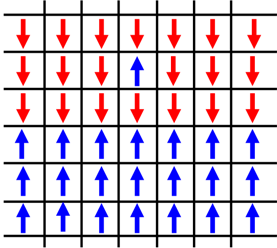
\includegraphics[width=0.4\textwidth]{ising.png}
  \label{fig:ising}
  \caption{\textbf{Schematic view of the Ising model.} Ising model schematic figure on a rectangular grid; blue arrows represent +1, red arrows represent -1 spins.}
 \end{center}

\end{figure}


\section{Results and discussion}

What to do if I'd like to include Table~\ref{table:ising}?

\begin{table}[h!]
  \begin{center}
    \begin{tabular}{lr}
    Color & Meaning\\ \hline
    blue & +1\\
    red & -1
  \end{tabular}
  \label{table:ising}
  \caption{Summary of color codings.}
  \end{center}
\end{table}


\subsection{This is a subsection}

\subsection{This is another subsection}

\section{Conclusion}

\clearpage

\bibliographystyle{plain}
\bibliography{sample}

\end{document}

